\documentclass{standalone}
\usepackage{tikz}
\usetikzlibrary{patterns, positioning}


\begin{document}
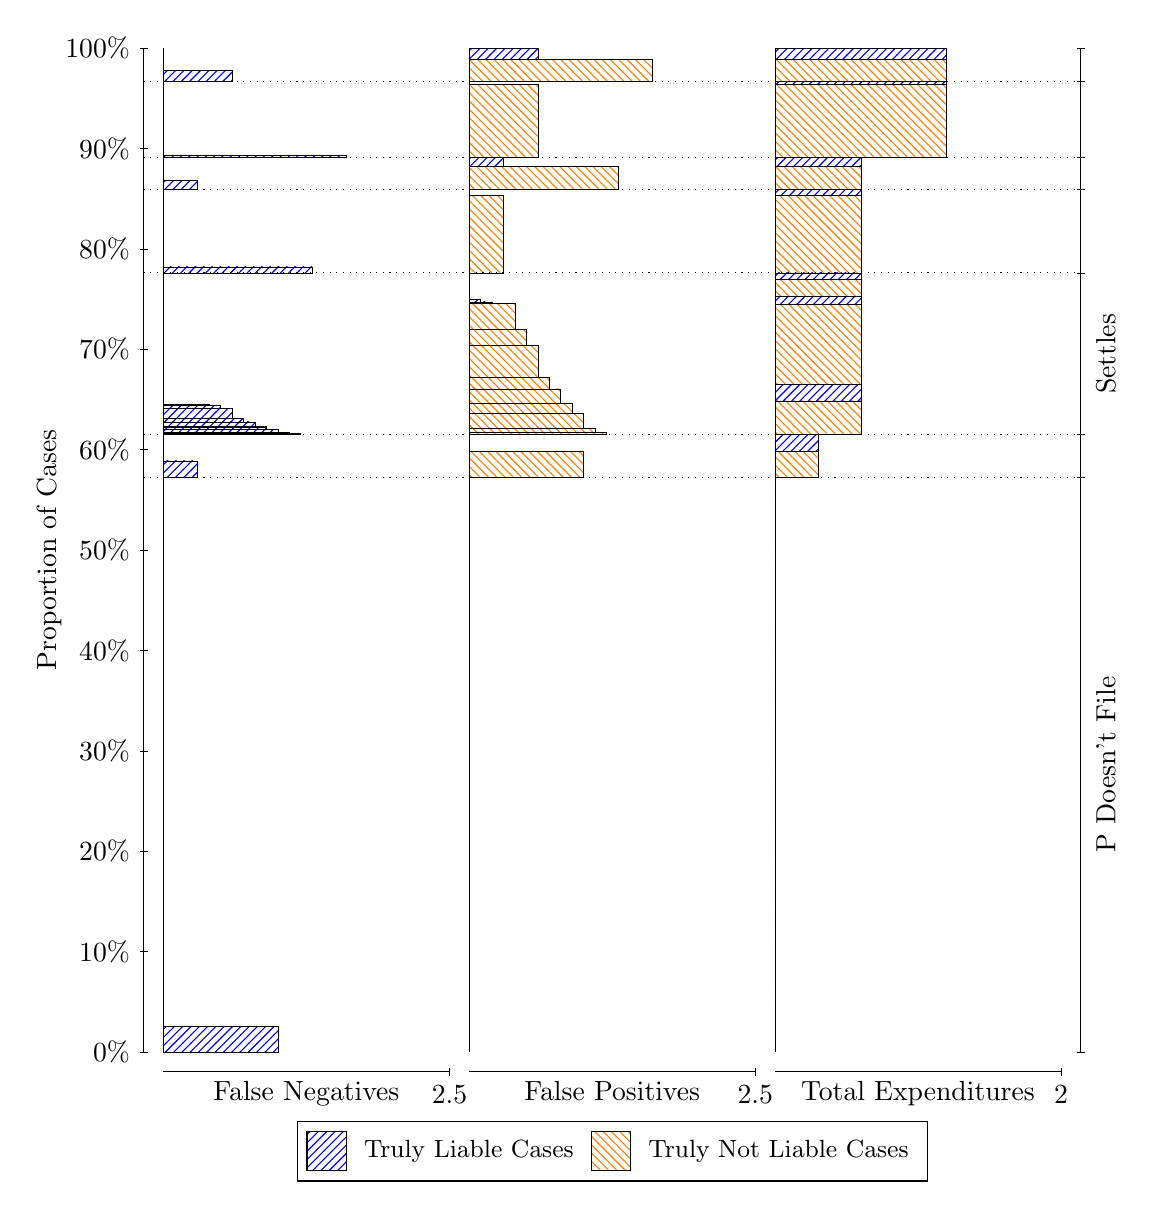
\begin{tikzpicture}
\draw[black, very thin] (1.5,1.75) -- (1.5,14.5);
\node[rotate=90, text=black, anchor=center] at (0.3, 8.125) {Proportion of Cases};
\draw[black, very thin] (1.45,1.75) -- (1.55,1.75);
\node[text=black, anchor=east] at (1.45, 1.75) {0\%};
\draw[black, very thin] (1.45,3.025) -- (1.55,3.025);
\node[text=black, anchor=east] at (1.45, 3.025) {10\%};
\draw[black, very thin] (1.45,4.3) -- (1.55,4.3);
\node[text=black, anchor=east] at (1.45, 4.3) {20\%};
\draw[black, very thin] (1.45,5.575) -- (1.55,5.575);
\node[text=black, anchor=east] at (1.45, 5.575) {30\%};
\draw[black, very thin] (1.45,6.85) -- (1.55,6.85);
\node[text=black, anchor=east] at (1.45, 6.85) {40\%};
\draw[black, very thin] (1.45,8.125) -- (1.55,8.125);
\node[text=black, anchor=east] at (1.45, 8.125) {50\%};
\draw[black, very thin] (1.45,9.4) -- (1.55,9.4);
\node[text=black, anchor=east] at (1.45, 9.4) {60\%};
\draw[black, very thin] (1.45,10.675) -- (1.55,10.675);
\node[text=black, anchor=east] at (1.45, 10.675) {70\%};
\draw[black, very thin] (1.45,11.95) -- (1.55,11.95);
\node[text=black, anchor=east] at (1.45, 11.95) {80\%};
\draw[black, very thin] (1.45,13.225) -- (1.55,13.225);
\node[text=black, anchor=east] at (1.45, 13.225) {90\%};
\draw[black, very thin] (1.45,14.5) -- (1.55,14.5);
\node[text=black, anchor=east] at (1.45, 14.5) {100\%};

\draw[black, very thin] (13.4,1.75) -- (13.4,14.5);
\draw[black, very thin] (13.35,1.75) -- (13.45,1.75);
\node[anchor=west] at (13.35, 1.75) {};
\draw[black, very thin] (13.35,9.0498) -- (13.45,9.0498);
\node[anchor=west] at (13.35, 9.0498) {};
\draw[black, very thin] (13.35,9.5885) -- (13.45,9.5885);
\node[anchor=west] at (13.35, 9.5885) {};
\draw[black, very thin] (13.35,11.644) -- (13.45,11.644);
\node[anchor=west] at (13.35, 11.644) {};
\draw[black, very thin] (13.35,12.706) -- (13.45,12.706);
\node[anchor=west] at (13.35, 12.706) {};
\draw[black, very thin] (13.35,13.109) -- (13.45,13.109);
\node[anchor=west] at (13.35, 13.109) {};
\draw[black, very thin] (13.35,14.074) -- (13.45,14.074);
\node[anchor=west] at (13.35, 14.074) {};
\draw[black, very thin] (13.35,14.5) -- (13.45,14.5);
\node[anchor=west] at (13.35, 14.5) {};

\draw[black, very thin, pattern color=blue, pattern=north east lines] (1.75,1.75) rectangle (3.2033,2.0756);
\draw[black, very thin, pattern color=orange, pattern=north west lines] (1.75,2.0756) rectangle (1.75,9.0498);
\draw[black, very thin, pattern color=blue, pattern=north east lines] (1.75,9.0498) rectangle (2.186,9.2564);
\draw[black, very thin, pattern color=orange, pattern=north west lines] (1.75,9.2564) rectangle (1.75,9.5885);
\draw[black, very thin, pattern color=blue, pattern=north east lines] (1.75,9.5885) rectangle (3.494,9.6062);
\draw[black, very thin, pattern color=blue, pattern=north east lines] (1.75,9.6062) rectangle (3.3487,9.6221);
\draw[black, very thin, pattern color=blue, pattern=north east lines] (1.75,9.6221) rectangle (3.2033,9.6549);
\draw[black, very thin, pattern color=blue, pattern=north east lines] (1.75,9.6549) rectangle (3.058,9.6808);
\draw[black, very thin, pattern color=blue, pattern=north east lines] (1.75,9.6808) rectangle (3.058,9.6956);
\draw[black, very thin, pattern color=blue, pattern=north east lines] (1.75,9.6956) rectangle (2.9127,9.7515);
\draw[black, very thin, pattern color=blue, pattern=north east lines] (1.75,9.7515) rectangle (2.7673,9.8003);
\draw[black, very thin, pattern color=blue, pattern=north east lines] (1.75,9.8003) rectangle (2.622,9.9267);
\draw[black, very thin, pattern color=blue, pattern=north east lines] (1.75,9.9267) rectangle (2.4767,9.9573);
\draw[black, very thin, pattern color=blue, pattern=north east lines] (1.75,9.9573) rectangle (2.3313,9.9713);
\draw[black, very thin, pattern color=orange, pattern=north west lines] (1.75,9.9713) rectangle (1.75,11.644);
\draw[black, very thin, pattern color=blue, pattern=north east lines] (1.75,11.644) rectangle (3.6393,11.721);
\draw[black, very thin, pattern color=orange, pattern=north west lines] (1.75,11.721) rectangle (1.75,12.706);
\draw[black, very thin, pattern color=blue, pattern=north east lines] (1.75,12.706) rectangle (2.186,12.816);
\draw[black, very thin, pattern color=orange, pattern=north west lines] (1.75,12.816) rectangle (1.75,13.109);
\draw[black, very thin, pattern color=blue, pattern=north east lines] (1.75,13.109) rectangle (4.0753,13.141);
\draw[black, very thin, pattern color=orange, pattern=north west lines] (1.75,13.141) rectangle (1.75,14.074);
\draw[black, very thin, pattern color=blue, pattern=north east lines] (1.75,14.074) rectangle (2.622,14.215);
\draw[black, very thin, pattern color=orange, pattern=north west lines] (1.75,14.215) rectangle (1.75,14.5);
\draw[black, very thin, pattern color=orange, pattern=north west lines] (5.6333,1.75) rectangle (5.6333,8.7242);
\draw[black, very thin, pattern color=blue, pattern=north east lines] (5.6333,8.7242) rectangle (5.6333,9.0498);
\draw[black, very thin, pattern color=orange, pattern=north west lines] (5.6333,9.0498) rectangle (7.0867,9.382);
\draw[black, very thin, pattern color=blue, pattern=north east lines] (5.6333,9.382) rectangle (5.6333,9.5885);
\draw[black, very thin, pattern color=orange, pattern=north west lines] (5.6333,9.5885) rectangle (7.3773,9.6165);
\draw[black, very thin, pattern color=orange, pattern=north west lines] (5.6333,9.6165) rectangle (7.232,9.6674);
\draw[black, very thin, pattern color=orange, pattern=north west lines] (5.6333,9.6674) rectangle (7.0867,9.8616);
\draw[black, very thin, pattern color=orange, pattern=north west lines] (5.6333,9.8616) rectangle (6.9413,9.9834);
\draw[black, very thin, pattern color=orange, pattern=north west lines] (5.6333,9.9834) rectangle (6.796,10.17);
\draw[black, very thin, pattern color=orange, pattern=north west lines] (5.6333,10.17) rectangle (6.6507,10.322);
\draw[black, very thin, pattern color=orange, pattern=north west lines] (5.6333,10.322) rectangle (6.5053,10.72);
\draw[black, very thin, pattern color=orange, pattern=north west lines] (5.6333,10.72) rectangle (6.36,10.929);
\draw[black, very thin, pattern color=orange, pattern=north west lines] (5.6333,10.929) rectangle (6.2147,11.261);
\draw[black, very thin, pattern color=blue, pattern=north east lines] (5.6333,11.261) rectangle (5.924,11.275);
\draw[black, very thin, pattern color=blue, pattern=north east lines] (5.6333,11.275) rectangle (5.7787,11.306);
\draw[black, very thin, pattern color=blue, pattern=north east lines] (5.6333,11.306) rectangle (5.6333,11.644);
\draw[black, very thin, pattern color=orange, pattern=north west lines] (5.6333,11.644) rectangle (6.0693,12.629);
\draw[black, very thin, pattern color=blue, pattern=north east lines] (5.6333,12.629) rectangle (5.6333,12.706);
\draw[black, very thin, pattern color=orange, pattern=north west lines] (5.6333,12.706) rectangle (7.5227,12.998);
\draw[black, very thin, pattern color=blue, pattern=north east lines] (5.6333,12.998) rectangle (6.0693,13.109);
\draw[black, very thin, pattern color=orange, pattern=north west lines] (5.6333,13.109) rectangle (6.5053,14.043);
\draw[black, very thin, pattern color=blue, pattern=north east lines] (5.6333,14.043) rectangle (5.6333,14.074);
\draw[black, very thin, pattern color=orange, pattern=north west lines] (5.6333,14.074) rectangle (7.9587,14.359);
\draw[black, very thin, pattern color=blue, pattern=north east lines] (5.6333,14.359) rectangle (6.5053,14.5);
\draw[black, very thin, pattern color=orange, pattern=north west lines] (9.5167,1.75) rectangle (9.5167,8.7242);
\draw[black, very thin, pattern color=blue, pattern=north east lines] (9.5167,8.7242) rectangle (9.5167,9.0498);
\draw[black, very thin, pattern color=orange, pattern=north west lines] (9.5167,9.0498) rectangle (10.062,9.382);
\draw[black, very thin, pattern color=blue, pattern=north east lines] (9.5167,9.382) rectangle (10.062,9.5885);
\draw[black, very thin, pattern color=orange, pattern=north west lines] (9.5167,9.5885) rectangle (10.607,10.02);
\draw[black, very thin, pattern color=blue, pattern=north east lines] (9.5167,10.02) rectangle (10.607,10.233);
\draw[black, very thin, pattern color=orange, pattern=north west lines] (9.5167,10.233) rectangle (10.607,11.249);
\draw[black, very thin, pattern color=blue, pattern=north east lines] (9.5167,11.249) rectangle (10.607,11.341);
\draw[black, very thin, pattern color=orange, pattern=north west lines] (9.5167,11.341) rectangle (10.607,11.566);
\draw[black, very thin, pattern color=blue, pattern=north east lines] (9.5167,11.566) rectangle (10.607,11.644);
\draw[black, very thin, pattern color=orange, pattern=north west lines] (9.5167,11.644) rectangle (10.607,12.629);
\draw[black, very thin, pattern color=blue, pattern=north east lines] (9.5167,12.629) rectangle (10.607,12.706);
\draw[black, very thin, pattern color=orange, pattern=north west lines] (9.5167,12.706) rectangle (10.607,12.998);
\draw[black, very thin, pattern color=blue, pattern=north east lines] (9.5167,12.998) rectangle (10.607,13.109);
\draw[black, very thin, pattern color=orange, pattern=north west lines] (9.5167,13.109) rectangle (11.697,14.043);
\draw[black, very thin, pattern color=blue, pattern=north east lines] (9.5167,14.043) rectangle (11.697,14.074);
\draw[black, very thin, pattern color=orange, pattern=north west lines] (9.5167,14.074) rectangle (11.697,14.359);
\draw[black, very thin, pattern color=blue, pattern=north east lines] (9.5167,14.359) rectangle (11.697,14.5);
\draw[black, dotted] (1.5,9.0498) -- (13.4,9.0498);
\draw[black, dotted] (1.5,9.5885) -- (13.4,9.5885);
\draw[black, dotted] (1.5,11.644) -- (13.4,11.644);
\draw[black, dotted] (1.5,12.706) -- (13.4,12.706);
\draw[black, dotted] (1.5,13.109) -- (13.4,13.109);
\draw[black, dotted] (1.5,14.074) -- (13.4,14.074);
\draw[black, very thin] (1.75,1.5) -- (5.3833,1.5);
\node[text=black, anchor=north] at (3.5667, 1.5) {False Negatives};
\draw[black, very thin] (5.3833,1.45) -- (5.3833,1.55);
\node[text=black, anchor=north] at (5.3833, 1.45) {2.5};

\draw[black, very thin] (5.6333,1.5) -- (9.2667,1.5);
\node[text=black, anchor=north] at (7.45, 1.5) {False Positives};
\draw[black, very thin] (9.2667,1.45) -- (9.2667,1.55);
\node[text=black, anchor=north] at (9.2667, 1.45) {2.5};

\draw[black, very thin] (9.5167,1.5) -- (13.15,1.5);
\node[text=black, anchor=north] at (11.333, 1.5) {Total Expenditures};
\draw[black, very thin] (13.15,1.45) -- (13.15,1.55);
\node[text=black, anchor=north] at (13.15, 1.45) {2};

\node[text=black, centered, rotate=90] at (13.72, 5.3999) {P Doesn't File};

\node[text=black, centered, rotate=90] at (13.72, 10.616) {Settles};





\draw (7.449999999999999,1.5) node[draw=none] (baseCoordinate) {};
\begin{scope}[align=center]
        \matrix[scale=0.5, draw=black, below=0.5cm of baseCoordinate, nodes={draw}, column sep=0.1cm]{
            \node[rectangle, draw, minimum width=0.5cm, minimum height=0.5cm, pattern color=blue, pattern=north east lines] {}; &
            \node[draw=none, font=\small, text=black] (B) {Truly Liable Cases}; &
            \node[rectangle, draw, minimum width=0.5cm, minimum height=0.5cm, pattern color=orange, pattern=north west lines] {}; &
            \node[draw=none, font=\small, text=black] (B) {Truly Not Liable Cases}; \\
            };
\end{scope}

\end{tikzpicture}
\end{document}